\documentclass[10pt,a4paper,twocolumn]{article}
\usepackage[utf8]{inputenc}
\usepackage[T1]{fontenc}
\usepackage[french]{babel}
\usepackage{lmodern}
\usepackage[a4paper,margin=1.65cm,columnsep=0.6cm]{geometry}
\usepackage{graphicx,booktabs,amsmath,array,xcolor,tikz,caption,enumitem}
\usepackage[hidelinks]{hyperref}
\usetikzlibrary{positioning,arrows.meta,fit}
\captionsetup{font=small,labelfont=bf,skip=3pt}
\setlist{nosep,leftmargin=*}
\setlength{\parskip}{0pt}
\setlength{\textfloatsep}{8pt plus 2pt minus 2pt}
\setlength{\floatsep}{6pt plus 2pt minus 2pt}
\setlength{\intextsep}{6pt plus 2pt minus 2pt}
\renewcommand{\arraystretch}{1.08}
\newcolumntype{L}[1]{>{\raggedright\arraybackslash}p{#1}}
\definecolor{olive}{RGB}{62,96,44}
\definecolor{retro}{RGB}{176,96,20}
\newcommand{\retro}{\textcolor{retro}{\textsuperscript{\textsf{R}}}}
\makeatletter
\renewcommand\section{\@startsection{section}{1}{\z@}{-1.6ex plus -.4ex}{0.7ex}{\normalfont\large\bfseries\color{olive}}}
\renewcommand\subsection{\@startsection{subsection}{2}{\z@}{-1.2ex plus -.3ex}{0.4ex}{\normalfont\normalsize\bfseries}}
\makeatother

\begin{document}

% ============================== PAGE DE GARDE ==============================
\onecolumn
\thispagestyle{empty}
\begin{center}
\vspace*{1.5cm}
{\large Rapport de projet --- Étape 1}\\[1.2cm]
{\Huge\bfseries\color{olive} OliveSmart --- OLV-6}\\[0.8cm]
{\LARGE Détection de la disparition apparente d'oliviers\\[0.2cm] sur images satellitaires multi-dates}\\[0.6cm]
{\large Comparaison de cinq méthodes sur un test spatial commun,\\ analyses rétrospectives et protocole de validation}\\[2.2cm]
{\large 5IIR --- Développement Digital et Système d'Information}\\[0.2cm]
{\large Framework J2EE et Architecture Microservices --- Deep Learning}\\[2.2cm]
{\large\bfseries Réalisé par :}\\[0.3cm]
{\large NAZIH Salma \quad GARTITE Yassine \quad TECHA Abderrahmane}\\[2.5cm]
{\large Année universitaire 2026--2027}\\[0.4cm]
{\normalsize Version révisée intégrant les remarques du jury et de la revue scientifique}
\end{center}
\clearpage
\twocolumn
\setcounter{page}{2}

% ================================ TITRE ===================================
\twocolumn[{%
\begin{center}
{\Large\bfseries Détection de la disparition apparente d'oliviers :\\ comparaison spatialement tenue à l'écart de cinq méthodes}\\[0.25cm]
{\small NAZIH Salma, GARTITE Yassine, TECHA Abderrahmane --- OliveSmart OLV-6}
\end{center}
\begin{small}
\noindent\textbf{Résumé ---} Nous comparons cinq méthodes pour repérer, à partir d'images satellitaires WorldView-2 de 2019, 2020
et 2021 (jeu OQDS), les oliviers dont la couronne \emph{disparaît} : seuil de variation, CUSUM, Isolation Forest, réseau siamois
convolutionnel (Siamese CNN) et réseau temporel convolutionnel (TCN). La cible est un \emph{proxy} de disparition apparente,
non un diagnostic sanitaire. Après contrôle qualité, 71\,956 arbres sont répartis par blocs spatiaux de 250\,m en entraînement,
validation et test (10\,205 arbres, 2,32\,\% de positifs). Dans la comparaison pré-spécifiée (phase~1), toutes les sélections sont
faites sur la validation et le test est ouvert une fois : le Siamese CNN obtient la meilleure PR-AUC (0,220) et le meilleur F1
(0,322), mais ne retrouve que 82 des 237 positifs. Des analyses \emph{rétrospectives} (phase~2), réalisées après consultation du
test et présentées comme telles, montrent que ce modèle était sous-entraîné : une version révisée (Siamese~v2, ensemble de
5 graines) atteint une PR-AUC de 0,486 (IC95 par blocs [0,11~;~0,73]) et un rappel de 72\,\%. Une validation croisée spatiale
(15 modèles, blocs de 250\,m à 1\,km) ramène l'estimation à $0{,}33\pm0{,}14$ pour un modèle seul : la performance ne dépend pas
de la taille des blocs mais varie fortement selon la zone. Une ablation indique que le gain provient de la comparaison des deux
dates et non d'un raccourci contextuel ; le modèle reste toutefois sensible aux variations d'éclairage. Le système reste un outil de priorisation des
inspections ; une validation géographique indépendante et une vérité terrain sont nécessaires avant tout usage.\\[0.1cm]
\textbf{Mots-clés ---} olivier ; télédétection ; détection de changement ; réseau siamois ; validation spatiale ; classes rares.
\end{small}
\vspace{0.35cm}
}]

% ============================ 1. INTRODUCTION =============================
\section{Introduction}
Le suivi sanitaire des oliveraies à grande échelle se heurte au coût des inspections visuelles. Le projet OliveSmart vise à
signaler automatiquement les arbres dont l'apparence change fortement entre deux acquisitions, afin d'orienter les visites.

Il faut distinguer trois niveaux : (i) la \emph{présence d'une couronne} sur l'image ; (ii) sa \emph{disparition apparente}
entre deux dates ; (iii) l'\emph{état phytosanitaire} réel de l'arbre. Dans OQDS~\cite{oqds}, la classe positive désigne un arbre
présent en 2019 puis absent des observations suivantes, interprété par les auteurs du jeu comme un retrait après infection
probable. Notre cible relève donc du niveau (ii) : c'est un proxy de disparition, pas un diagnostic. Un arbre malade mais encore
visible est un négatif, et un arbre retiré pour une autre cause est un positif. Cette distinction est maintenue dans tout le
rapport : « positif » signifie toujours « disparition apparente selon OQDS ».

\textbf{Lacune et hypothèse.} Comparer un modèle qui voit des images RGB à des méthodes qui ne voient que des statistiques
résumées confond deux effets : l'algorithme et l'information d'entrée. Un écart de performance ne peut donc pas être attribué
au seul modèle. Nous traitons cette question explicitement par une ablation contrôlée (section~\ref{sec:ablation}).

\textbf{Questions de recherche.} \textbf{RQ1} : une comparaison visuelle de deux dates apporte-t-elle plus d'information que des
indicateurs radiométriques agrégés ? \textbf{RQ2} : quel compromis entre rappel, fausses alertes et charge d'inspection ?
\textbf{RQ3} : les performances sont-elles favorisées par des pixels noirs ou des régions invalides ?

\textbf{Contributions.} (1) Un audit des données et de l'étiquette indirecte, avec ventilation des exclusions et contrôle de la
dépendance spatiale ; (2) une comparaison de cinq méthodes sur une population de test commune, avec seuils fixés sur la
validation ; (3) la traduction des scores en nombres d'inspections, d'alertes fausses et d'omissions. Nous ne revendiquons ni une
nouvelle architecture, ni une détection de maladie confirmée.

\textbf{Organisation.} La section~2 situe les travaux connexes, la section~3 décrit les données, la section~4 les méthodes et le
protocole en deux phases, la section~5 les résultats pré-spécifiés, la section~6 les analyses rétrospectives, la section~7 la
discussion et la section~8 le protocole de validation futur.

% =========================== 2. TRAVAUX CONNEXES ==========================
\section{Travaux connexes}
Trois courants encadrent l'étude : la cartographie et le suivi sanitaire de l'olivier, qui distinguent localiser une couronne,
reconnaître un symptôme et constater une disparition ; les méthodes de comparaison d'images multi-dates ; et l'évaluation sous
dépendance spatiale et classes rares.

\textbf{Olivier.} Lin et al.~\cite{lin} cartographient les oliviers existants : l'unité est l'arbre, mais sans suivi temporel
individuel. Raouhi et al.~\cite{raouhi} classent des maladies à partir de photographies de feuilles, avec des images et une cible
sans rapport avec la télédétection. OQDS~\cite{oqds} fournit au contraire des points d'arbres suivis sur trois dates.

\textbf{Détection de changement.} CUSUM~\cite{page} cumule les écarts pour détecter une rupture ; Isolation Forest~\cite{iforest}
isole les observations atypiques. Les réseaux siamois~\cite{bromley} encodent deux entrées par un réseau commun ; Daudt et
al.~\cite{daudt} les appliquent à la segmentation du changement \emph{pixel par pixel}, alors que nous produisons une étiquette
\emph{par arbre}. Les TCN~\cite{bai} sont conçus pour des séries longues ; ici la série ne compte que trois dates, ce qui en limite
l'intérêt (section~\ref{sec:ablation}).

\textbf{Validation spatiale et classes rares.} Des observations voisines partagent sol, éclairage et acquisition ; une
validation aléatoire surestime alors les performances~\cite{roberts}. Les blocs spatiaux et les zones tampons sont
recommandés~\cite{valavi}. Pour des positifs rares, la courbe précision--rappel est plus informative que l'accuracy ou la courbe
ROC~\cite{saito}.

\begin{table}[t]
\centering\small
\caption{Positionnement : les tâches diffèrent par l'unité prédite et la cible ; leurs scores ne sont pas comparables.}
\label{tab:related}
\setlength{\tabcolsep}{3pt}
\begin{tabular}{@{}L{1.5cm}L{1.0cm}L{2.75cm}L{1.0cm}@{}}
\toprule
Travail & Unité & Cible & Dates \\
\midrule
Lin~\cite{lin} & arbre & présence de l'arbre & une \\
Raouhi~\cite{raouhi} & feuille & maladie foliaire & une \\
Daudt~\cite{daudt} & pixel & carte de changement & deux \\
\textbf{OLV-6} & \textbf{arbre} & \textbf{disparition apparente} & \textbf{trois} \\
\bottomrule
\end{tabular}
\end{table}

\textbf{Synthèse.} Ces travaux ne constituent pas des références directement comparables : la cartographie localise des
arbres existants, la classification foliaire utilise d'autres images, la détection de changement prédit à l'échelle du pixel.
Notre contribution est une comparaison \emph{interne au corpus}, sur des identités d'arbres alignées, et non une revendication
d'état de l'art.

% ============================== 3. DONNÉES ================================
\section{Données}
\textbf{Sources et choix d'OQDS.} La Table~\ref{tab:datasets} résume les quatre sources de l'énoncé. OQDS est retenu comme
source principale car c'est la seule qui associe, pour chaque arbre, une position géoréférencée et trois acquisitions
co-enregistrées au même capteur et à la même résolution. Seule cette combinaison permet une classification \emph{par arbre} et
\emph{dans le temps}. Ses limites sont fortes : l'étiquette ne décrit qu'une disparition apparente ; la zone couvre environ
35\,km$^2$ d'un seul secteur ; il n'y a que trois dates ; et les images sont des produits RGB 8 bits sans proche infrarouge
calibré. Les trois autres sources servent d'audit ou d'expérience exploratoire, pas de test équivalent.

\begin{table*}[t]
\centering\small
\caption{Caractéristiques des quatre sources étudiées.}
\label{tab:datasets}
\setlength{\tabcolsep}{4pt}
\begin{tabular}{@{}lL{2.6cm}L{3.3cm}L{3.4cm}L{2.0cm}L{2.3cm}@{}}
\toprule
Source & Taille & Imagerie / résolution & Annotation & Période & Usage ici \\
\midrule
OQDS~\cite{oqds} & 77\,086 points d'arbres (71\,956 retenus) & WorldView-2, RGB + rendu « NDVI » RGBA 8 bits ; 0,5\,m ; $14\,462\times9\,727$ px ($\approx$35\,km$^2$) & point par arbre ; présent en 2019 puis absent (disparition apparente) & 2019, 2020, 2021 & benchmark principal \\
NEON~\cite{neon} & 41\,738 couronnes ; 38 sites ; 234 taxons & polygones de couronnes issus d'imagerie aéroportée & espèce, hauteur, statut (souvent manquant) & 2017--2024 (années d'annotation/détection) & audit : aucune paire d'années exploitable par individu \\
Hyperspectral~\cite{hyper} & 76 oliviers & cubes $50\times50$ px, 138 bandes & stress à \emph{Verticillium} ; 6 infections « possibles » & une campagne & expérience exploratoire de stress \\
CrownsDb~\cite{crowns} & 5\,844 images drone, 33\,479 boîtes & RGB drone, de $5\,472\times3\,648$ à $608\times405$ px & boîtes de couronnes (une classe) & aucune information temporelle & audit qualité des couronnes \\
\bottomrule
\end{tabular}
\end{table*}

\textbf{Images dites « NDVI ».} Les fichiers nommés NDVI dans OQDS sont des \emph{rendus RGBA 8 bits}, sans bande proche
infrarouge calibrée. Leurs intensités sont utilisées comme caractéristiques d'image et ne peuvent pas être interprétées comme un
indice de végétation physique ni comme une mesure de la physiologie de l'arbre.

\textbf{Contrôle qualité.} Le catalogue compte 77\,086 points. Après suppression de 104 doublons géométriques, 5\,026
observations invalides sont \emph{exclues} (et non réétiquetées négatives), ce qui laisse 71\,956 arbres
(Table~\ref{tab:qc}). Les exclus sont moins souvent positifs (1,95\,\% contre 2,88\,\% ; $\chi^2$, $p=1{,}5\cdot10^{-4}$) : le
filtrage écarte 98 positifs (4,5\,\%) et enrichit légèrement la population retenue. Ce biais de sélection est modeste mais réel.

\begin{table}[t]
\centering\small
\caption{Exclusions par motif et par classe (après déduplication).}
\label{tab:qc}
\setlength{\tabcolsep}{4pt}
\begin{tabular}{@{}lrrr@{}}
\toprule
Motif & Négatifs & Positifs & Prév. \\
\midrule
Conservés & 69\,887 & 2\,069 & 2,88\,\% \\
RGB majoritairement noir & 4\,861 & 98 & 1,98\,\% \\
Couverture alpha insuffisante & 59 & 0 & 0\,\% \\
Hors raster / bord de patch & 8 & 0 & 0\,\% \\
\midrule
Total exclu & 4\,928 & 98 & 1,95\,\% \\
\bottomrule
\end{tabular}
\end{table}

\textbf{Partition spatiale.} Les arbres sont regroupés en blocs de 250\,m, chaque bloc étant affecté à une seule partition
(StratifiedGroupKFold, 7 folds ; fold~0 = test, fold~5 = validation). Aucun arbre ni bloc n'est partagé, mais des blocs
\emph{adjacents} peuvent l'être : la distance minimale entre un arbre test et un arbre d'entraînement est de 1,6\,m, la médiane
de 62\,m, et 12\,\% des arbres test sont à moins de 16\,m d'un arbre d'entraînement. Le risque de fuite est évalué en
section~\ref{sec:leak}. Les positifs sont très concentrés (Table~\ref{tab:split}) : ceux du test se trouvent dans 5 blocs sur
52, avec jusqu'à 62\,\% de positifs dans un bloc. Les scores de test dépendent donc de quelques zones, ce qui explique
l'écart validation/test et la largeur des intervalles de confiance.

\textbf{Différences radiométriques entre dates.} Sur 20\,000 arbres négatifs, la luminance moyenne des patches vaut 165 en
2019, 176 en 2020 et 168 en 2021 (échelle 0--255). L'image de 2020 est donc nettement plus claire, et la part de pixels sombres
(luminance $<60$, indicateur d'ombre) y tombe à 1,4\,\%, contre 2,3\,\% en 2019 et 2,1\,\% en 2021. Ces écarts varient selon
les zones : par bloc, la variation médiane de luminance de 2019 à 2021 va de $-6$ à $+10$ (déciles 10--90\,\%), et de $-28$ à
$+5$ entre 2020 et 2021 (Figure~\ref{fig:radio}). Un arbre négatif peut donc « changer » d'apparence sans aucune disparition.
C'est la principale source de fausses alertes des méthodes fondées sur l'intensité (section~\ref{sec:fp}). Les acquisitions
ne sont pas datées précisément dans OQDS : l'effet saisonnier ne peut pas être séparé de l'effet capteur et éclairage.

\begin{figure}[t]
\centering
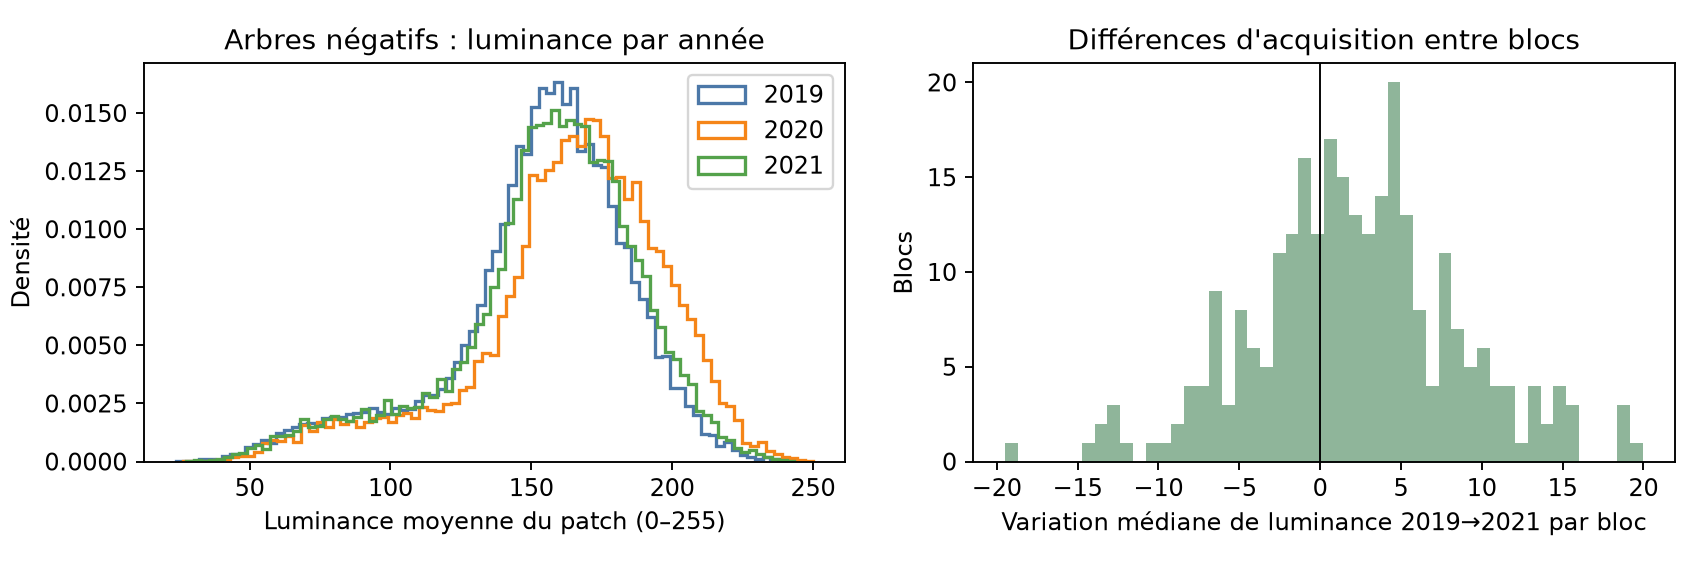
\includegraphics[width=\columnwidth]{figures/radiometrie.png}
\caption{Radiométrie des arbres négatifs. Gauche : luminance des patches par année. Droite : variation médiane de luminance
2019$\to$2021 par bloc spatial (différences d'acquisition entre zones).}
\label{fig:radio}
\end{figure}

\begin{table}[t]
\centering\small
\caption{Partitions spatiales et concentration des positifs.}
\label{tab:split}
\setlength{\tabcolsep}{3.5pt}
\begin{tabular}{@{}lrrrrr@{}}
\toprule
Partition & Arbres & Positifs & Prév. & Blocs & Blocs pos. \\
\midrule
Entraînement & 51\,425 & 1\,541 & 3,00\,\% & 258 & 36 \\
Validation & 10\,326 & 291 & 2,82\,\% & 53 & 10 \\
Test & 10\,205 & 237 & 2,32\,\% & 52 & 5 \\
\bottomrule
\end{tabular}
\end{table}

% ============================= 4. MÉTHODES ================================
\section{Méthodes et protocole}
\subsection{Représentations et modèles}
Les cinq méthodes ne reçoivent pas la même information ; le classement compare donc des \emph{chaînes complètes}
(représentation + modèle), non des architectures isolées.
\begin{itemize}
\item \textbf{Seuil} : score de baisse d'intensité entre dates (baisse totale, annuelle maximale ou relative).
\item \textbf{CUSUM}~\cite{page} : cumul des baisses au-delà d'une tolérance $k$, absolu ou relatif.
\item \textbf{Isolation Forest}~\cite{iforest} : anomalie sur les statistiques d'intensité tabulaires, ajusté sur les négatifs
d'entraînement.
\item \textbf{TCN}~\cite{bai} : 4 statistiques (moyenne, écart-type, percentiles 10 et 90) $\times$ 3 dates ; deux blocs résiduels.
\item \textbf{Siamese CNN}~\cite{bromley} : patches RGB de 16$\times$16 pixels (8\,m) centrés sur l'arbre en 2019 et 2021, un
encodeur à poids partagés, puis fusion $[|z_a-z_b|,\; z_a\odot z_b,\; z_b-z_a]$ et classifieur.
\end{itemize}
Les deux réseaux utilisent une entropie croisée pondérée. Toute normalisation est ajustée sur l'entraînement seul. La
Table~\ref{tab:arch} détaille les architectures.

\begin{table*}[t]
\centering\small
\caption{Architectures des réseaux (activations ReLU ; GAP : moyenne globale ; BN : normalisation par lots).}
\label{tab:arch}
\begin{tabular}{@{}lL{2.0cm}L{6.3cm}L{3.6cm}r@{}}
\toprule
Modèle & Entrée & Encodeur / corps & Fusion et tête & Param. \\
\midrule
Siamese initial & $2\times(3\times16\times16)$ & Conv 3$\times$3 (16) -- MaxPool -- Conv 3$\times$3 (32) -- GAP $\to$ 32 ; poids partagés & $[|z_a-z_b|, z_a\odot z_b]$ (64) $\to$ 32 -- Dropout 0,35 $\to$ 1 & 7\,201 \\
Siamese v2 & $2\times(3\times32\times32)$ & 3 blocs [Conv 3$\times$3 -- BN -- ReLU]$\times$2 à 16, 32, 64 canaux, MaxPool entre blocs, GAP $\to$ 64 ; poids partagés & $[|z_a-z_b|, z_a\odot z_b, z_b-z_a]$ (192) $\to$ 64 -- Dropout 0,3 $\to$ 1 & 84\,721 \\
TCN & $4\times3$ (statistiques $\times$ dates) & 2 blocs résiduels causaux : Conv1d noyau 2, 12 canaux, dilatations 1 puis 2, Dropout 0,1, saut 1$\times$1 & sortie du dernier pas $\to$ 1 & 1\,081 \\
MLP (contrôle) & 12 & -- & 12 $\to$ 32 -- Dropout 0,1 $\to$ 1 & 449 \\
\bottomrule
\end{tabular}
\end{table*}

\subsection{Budgets de recherche}
La Table~\ref{tab:hp} détaille les grilles. Les budgets sont petits et non uniformes : trois variantes par famille, et six pour
CUSUM car deux paramètres (mode et $k$) y sont croisés. Les réseaux sont entraînés un nombre fixe d'époques (6 pour le
Siamese, 8 pour le TCN) en gardant le checkpoint de meilleure PR-AUC de validation. Pour chaque méthode, le seuil de décision
maximise le F1 de validation.

\begin{table*}[t]
\centering\small
\caption{Phase 1 --- grilles explorées et configuration retenue (en gras) ; sélection sur la PR-AUC de validation, seuil
maximisant le F1 de validation.}
\label{tab:hp}
\begin{tabular}{@{}lcL{8.6cm}r@{}}
\toprule
Méthode & Essais & Variantes explorées & PR-AUC val. \\
\midrule
Seuil & 3 & baisse totale 2019--2021 ; \textbf{baisse annuelle maximale} ; baisse relative & 0,054 \\
CUSUM & 6 & mode absolu, $k\in\{0;\,5;\,\mathbf{10}\}$ ; mode relatif, $k\in\{0;\,0{,}03;\,0{,}06\}$ & 0,053 \\
Isolation Forest & 3 & (arbres, échantillons, part des variables) : (150, 256, 0,7) ; (250, 512, 1,0) ; \textbf{(350, 1024, 0,8)} & 0,030 \\
TCN & 3 & (lr, canaux, dropout, noyau) : \textbf{($10^{-3}$, 12, 0,10, 2)} ; ($4\cdot10^{-4}$, 20, 0,25, 2) ; ($7\cdot10^{-4}$, 16, 0,35, 3) ; 8 époques & 0,049 \\
Siamese CNN & 3 & (lr, largeur, dropout) : ($10^{-3}$, 8, 0,15) ; ($4\cdot10^{-4}$, 12, 0,25) ; \textbf{($7\cdot10^{-4}$, 16, 0,35)} ; 6 époques & 0,167 \\
\bottomrule
\end{tabular}
\end{table*}

\subsection{Protocole en deux phases}
\label{sec:proto}
La Figure~\ref{fig:proto} résume le protocole. En \textbf{phase~1} (pré-spécifiée), configurations, checkpoints et seuils sont
choisis sur la validation, puis le test est évalué \emph{une seule fois}. Ce sont les seuls résultats confirmatoires du rapport.
La \textbf{phase~2} regroupe les analyses faites \emph{après} consultation du test : Siamese~v2, graines multiples, intervalles
de confiance, contrôle de fuite et ablation. Le v2 a lui aussi été sélectionné sur la validation et évalué une fois. Mais comme
le test avait déjà été consulté, ses scores sont \textbf{rétrospectifs} et ne constituent pas une confirmation indépendante. Ils
sont marqués d'un \retro{} dans les tableaux.

\begin{figure}[t]
\centering
\begin{tikzpicture}[font=\scriptsize, node distance=2.5mm,
  b/.style={draw, rounded corners=2pt, align=center, minimum height=6.5mm, inner sep=2pt, fill=white},
  a/.style={-{Stealth[length=1.6mm]}}]
\node[b, fill=olive!12] (d) {OQDS\\71\,956 arbres};
\node[b, right=of d] (s) {Blocs 250\,m\\Train / Val / Test};
\node[b, right=of s, fill=olive!12] (v) {Sélection\\sur Val (PR-AUC)};
\node[b, below=4mm of v, fill=olive!25] (t) {\textbf{Test ouvert}\\\textbf{une fois} (phase 1)};
\node[b, left=of t, fill=retro!15, text width=2.9cm] (r) {Phase 2 rétrospective : v2, graines, IC, fuite, ablation};
\node[b, left=of r, fill=gray!12, text width=1.35cm] (f) {Futur : région scellée};
\draw[a] (d) -- (s); \draw[a] (s) -- (v); \draw[a] (v) -- (t); \draw[a] (t) -- (r);
\draw[a, dashed] (r) -- (f);
\end{tikzpicture}
\caption{Protocole : seule la phase 1 est confirmatoire. La phase 2 est un diagnostic rétrospectif ; une confirmation exige
une région nouvelle, scellée avant ouverture (section~\ref{sec:future}).}
\label{fig:proto}
\end{figure}

\textbf{Indicateurs.} Le critère principal est la PR-AUC, dont la valeur du hasard égale la prévalence (2,32\,\% en test). Nous
rapportons aussi la ROC-AUC (ordre des scores, indépendant du seuil), puis la précision, le rappel et le F1 \emph{au seuil fixé
sur validation}, ainsi que les nombres de vrais positifs (VP), faux positifs (FP) et faux négatifs (FN). Les intervalles de
confiance (IC95) sont obtenus par bootstrap des \emph{blocs spatiaux} du test (1\,000 tirages), et les comparaisons entre
modèles par bootstrap apparié sur les mêmes blocs.

% ======================= 5. RÉSULTATS PHASE 1 =============================
\section{Résultats pré-spécifiés (phase 1)}
La Table~\ref{tab:main} classe les cinq méthodes avec des mesures indépendantes du seuil (ROC-AUC, PR-AUC), puis avec des
mesures au seuil retenu. La Table~\ref{tab:burden} convertit ces décisions en charge opérationnelle. La distinction est
essentielle : une ROC-AUC correcte peut coexister avec un nombre excessif de fausses alertes.

\begin{table*}[t]
\centering\small
\caption{Phase 1 --- performances sur les 10\,205 arbres test (237 positifs). Seuils fixés sur validation. IC95 : bootstrap par
blocs spatiaux. Temps CPU sans GPU ; l'inférence est mesurée par lot sur les 10\,205 arbres (patches déjà extraits), ce n'est pas
une latence de requête unitaire. Le temps d'entraînement des réseaux inclut la recherche d'hyperparamètres.}
\label{tab:main}
\begin{tabular}{@{}l cc c ccc c rr@{}}
\toprule
& \multicolumn{3}{c}{Indépendant du seuil} & \multicolumn{4}{c}{Au seuil fixé sur validation} & \multicolumn{2}{c}{Temps CPU (s)} \\
\cmidrule(lr){2-4}\cmidrule(lr){5-8}\cmidrule(lr){9-10}
Méthode & ROC-AUC & PR-AUC & IC95 PR-AUC & Précision & Rappel & F1 & Accuracy & Entr. & Inf. (lot) \\
\midrule
\textbf{Siamese CNN} & \textbf{0,874} & \textbf{0,220} & [0,032 ; 0,442] & \textbf{0,301} & 0,346 & \textbf{0,322} & 0,966 & 70,7 & 0,396 \\
TCN & 0,763 & 0,062 & [0,007 ; 0,147] & 0,055 & \textbf{0,692} & 0,103 & 0,719 & 21,3 & 0,056 \\
CUSUM & 0,652 & 0,039 & [0,006 ; 0,090] & 0,047 & 0,143 & 0,071 & 0,913 & 0,06 & 0,0003 \\
Seuil & 0,625 & 0,033 & [0,005 ; 0,078] & 0,032 & 0,068 & 0,044 & 0,932 & 0,04 & 0,0001 \\
Isolation Forest & 0,556 & 0,026 & [0,004 ; 0,057] & 0,027 & \textbf{0,692} & 0,051 & 0,407 & 1,68 & 0,178 \\
\bottomrule
\end{tabular}
\end{table*}

\begin{table}[t]
\centering\small
\caption{Phase 1 --- charge d'alerte au seuil retenu (mêmes 237 positifs). « Alertes/VP » : nombre d'arbres à inspecter pour
trouver une disparition réelle.}
\label{tab:burden}
\setlength{\tabcolsep}{3.5pt}
\begin{tabular}{@{}lrrrrr@{}}
\toprule
Méthode & VP & FP & FN & Alertes & Alertes/VP \\
\midrule
Siamese CNN & 82 & 190 & 155 & 272 & 3,3 \\
TCN & 164 & 2\,795 & 73 & 2\,959 & 18,0 \\
Isolation Forest & 164 & 5\,975 & 73 & 6\,139 & 37,4 \\
CUSUM & 34 & 684 & 203 & 718 & 21,1 \\
Seuil & 16 & 478 & 221 & 494 & 30,9 \\
\bottomrule
\end{tabular}
\end{table}

\textbf{Siamese CNN.} Parmi les cinq chaînes testées, il obtient la meilleure PR-AUC, la meilleure ROC-AUC et le meilleur F1.
Au seuil retenu, il déclenche 272 alertes sur 10\,205 arbres : 82 correctes et 190 fausses, et laisse 155 positifs non détectés.
Son avantage de PR-AUC est significatif face à chaque autre méthode (bootstrap apparié par blocs : $+0{,}15$ [0,02~;~0,31] sur le
TCN, $+0{,}18$ [0,02~;~0,36] sur CUSUM, $+0{,}18$ [0,02~;~0,37] sur le seuil, $+0{,}19$ [0,02~;~0,39] sur Isolation Forest).
Ce classement relatif ne fait pas de lui un détecteur suffisamment sensible pour un usage sans contrôle humain.

\textbf{Il ne domine pas toutes les métriques.} Le TCN et Isolation Forest atteignent un rappel de 0,692 (164 positifs
retrouvés), supérieur à celui du Siamese (0,346), au prix de 2\,795 et 5\,975 fausses alertes : il faudrait inspecter 18 et
37 arbres par disparition réelle, contre 3,3. Le seuil et CUSUM sont très conservateurs ; leur accuracy élevée ne fait que
refléter la classe majoritaire. Le choix entre ces profils dépend du quota de visites et du coût d'une omission
(section~\ref{sec:op}).

\textbf{Pourquoi le TCN produit autant de fausses alertes.}
\label{sec:fp}
Le TCN ne voit que des statistiques d'intensité du rendu « NDVI ». Or l'intensité des arbres \emph{négatifs} baisse
différemment selon les zones (Table~\ref{tab:fp}). Parmi les négatifs, le score du TCN est fortement corrélé à cette baisse
($r=-0{,}72$), et 99,5\,\% de ses fausses alertes concernent des arbres dont l'intensité diminue. Dans le quart des blocs où
la baisse est la plus forte, il signale à tort 41\,\% des arbres ; le Siamese~v2\retro{}, qui compare la forme des couronnes,
n'en signale que 5\,\%. Le TCN confond donc un changement d'acquisition avec une disparition. Pour réduire ces alertes, il
faudrait normaliser l'intensité par rapport aux arbres voisins du même bloc (variation relative locale) ou ajouter une
information de forme.

\begin{table}[t]
\centering\small
\caption{Taux de fausses alertes sur les négatifs du test, par quartile de variation d'intensité de leur bloc (2019$\to$2021).}
\label{tab:fp}
\setlength{\tabcolsep}{3.5pt}
\begin{tabular}{@{}lrrrr@{}}
\toprule
Quartile (variation médiane) & Négatifs & FP TCN & FP v2\retro{} \\
\midrule
Q1 : baisse forte ($-52$) & 2\,573 & 41,3\,\% & 5,4\,\% \\
Q2 ($-47$) & 2\,511 & 29,7\,\% & 1,8\,\% \\
Q3 ($-42$) & 2\,493 & 24,0\,\% & 3,5\,\% \\
Q4 : baisse faible ($-31$) & 2\,391 & 16,2\,\% & 1,3\,\% \\
\bottomrule
\end{tabular}
\end{table}

\begin{figure}[t]
\centering
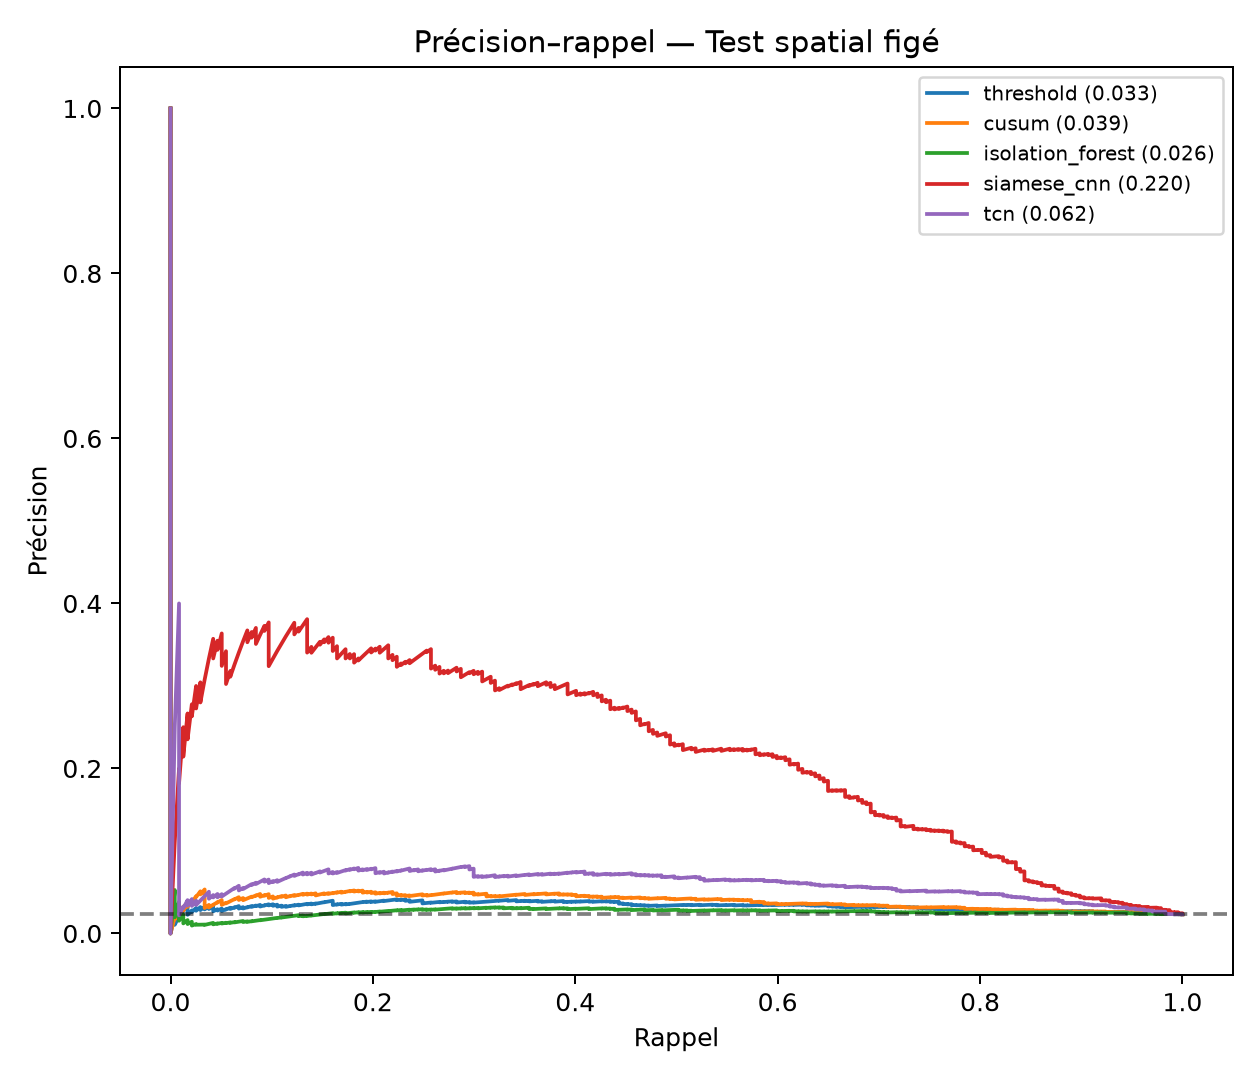
\includegraphics[width=0.92\columnwidth]{figures/precision_recall_curves_test.png}
\caption{Phase 1 --- courbes précision--rappel sur le test. Ligne pointillée : prévalence (2,32\,\%), valeur d'un classement
aléatoire pour la PR-AUC uniquement (elle n'est pas une référence pour le F1).}
\label{fig:pr1}
\end{figure}

% ======================= 6. ANALYSES RÉTROSPECTIVES ========================
\section{Analyses rétrospectives (phase 2)}
Toutes les analyses de cette section ont été faites après consultation du test (section~\ref{sec:proto}). Elles servent à
\emph{diagnostiquer} les résultats de la phase~1, non à les confirmer.

\subsection{Variabilité et Siamese v2}
\textbf{Variabilité entre graines.} Réentraînées avec 5 graines, les configurations de la phase~1 donnent une PR-AUC test de
$0{,}215\pm0{,}039$ pour le Siamese, $0{,}058\pm0{,}004$ pour le TCN et $0{,}027\pm0{,}001$ pour Isolation Forest : le classement
ne dépend pas d'une graine favorable.

\textbf{Sous-entraînement.} Avec 6 époques fixes, la PR-AUC de validation du Siamese augmentait encore en fin d'entraînement.
La même architecture, entraînée plus longtemps, passe de 0,167 à 0,228 en validation. Nous avons donc évalué sur la
\emph{validation} quatre configurations révisées. La meilleure (Siamese~v2, 0,293 avec la graine 0) comporte trois blocs
convolutifs avec normalisation par lots, des patches de 32$\times$32 pixels (16\,m), une augmentation géométrique identique
pour les deux dates (rotations de 90°, symétries) et une variation radiométrique indépendante par date. L'entraînement utilise
AdamW, une entropie croisée pondérée par $\sqrt{n_-/n_+}$, une réduction du pas sur plateau et un arrêt anticipé (patience 7,
au plus 40 époques). Le modèle compte 84\,721 paramètres. La PR-AUC de validation fluctuant d'une époque à l'autre
(Figure~\ref{fig:lc}), les scores de 5 graines sont moyennés (ensemble).

\textbf{Taille des patches.} Avec la même architecture, des patches de 16$\times$16 pixels (8\,m) donnent 0,265 en validation,
contre 0,293 en 32$\times$32 (16\,m). Le contexte autour de l'arbre aide : les couronnes voisines servent de référence
d'éclairage et d'échelle, et une couronne de grande taille ou légèrement décalée reste entièrement dans le patch.

\begin{figure*}[t]
\centering
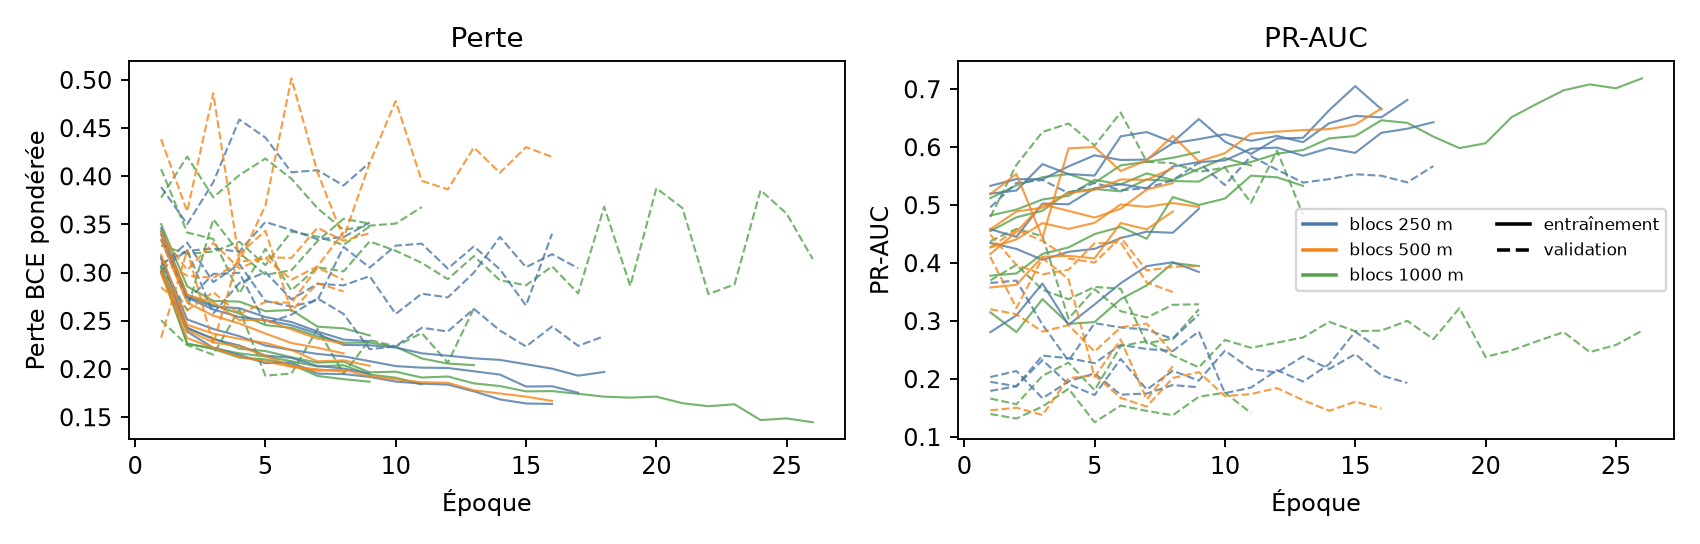
\includegraphics[width=0.86\textwidth]{figures/curves_cv.png}
\caption{Courbes d'apprentissage\retro{} du Siamese v2 pour les 15 entraînements de la validation croisée spatiale (traits pleins :
entraînement, PR-AUC mesurée sur 10\,000 arbres d'entraînement ; pointillés : validation). La PR-AUC d'entraînement continue de
monter (0,6--0,7) alors que celle de validation plafonne et fluctue : l'arrêt anticipé sur la validation limite le
surapprentissage. Les historiques de toutes les configurations sont fournis dans le dépôt.}
\label{fig:lc}
\end{figure*}

\begin{table}[t]
\centering\small
\caption{Siamese v2\retro{} contre Siamese initial (test). Seuil v2 fixé sur validation (0,72).}
\label{tab:v2}
\footnotesize
\setlength{\tabcolsep}{2.5pt}
\begin{tabular}{@{}lcc@{}}
\toprule
& Siamese initial & Siamese v2\retro{} \\
\midrule
PR-AUC validation & 0,167 & 0,314 \\
PR-AUC, 5 graines & $0{,}215\pm0{,}039$ & $0{,}468\pm0{,}050$ \\
PR-AUC ensemble & 0,220 & 0,486 \\
\quad IC95 & [0,03 ; 0,44] & [0,11 ; 0,73] \\
ROC-AUC ensemble & 0,874 & 0,961 \\
\quad IC95 & [0,77 ; 0,91] & [0,93 ; 0,98] \\
Précision / rappel & 0,301 / 0,346 & 0,362 / 0,722 \\
F1 & 0,322 & 0,482 \\
VP / FP / FN & 82 / 190 / 155 & 171 / 302 / 66 \\
\bottomrule
\end{tabular}
\end{table}

Le v2 retrouve 171 positifs au lieu de 82 et divise les omissions par 2,3, au prix de 112 alertes supplémentaires
(Table~\ref{tab:v2}, Figure~\ref{fig:pr2}). Le gain apparié de PR-AUC sur le Siamese initial est de $+0{,}24$ [0,08~;~0,35].
L'IC95 du v2 reste toutefois très large, conséquence directe des 5 blocs qui contiennent tous les positifs du test.

\begin{figure}[t]
\centering
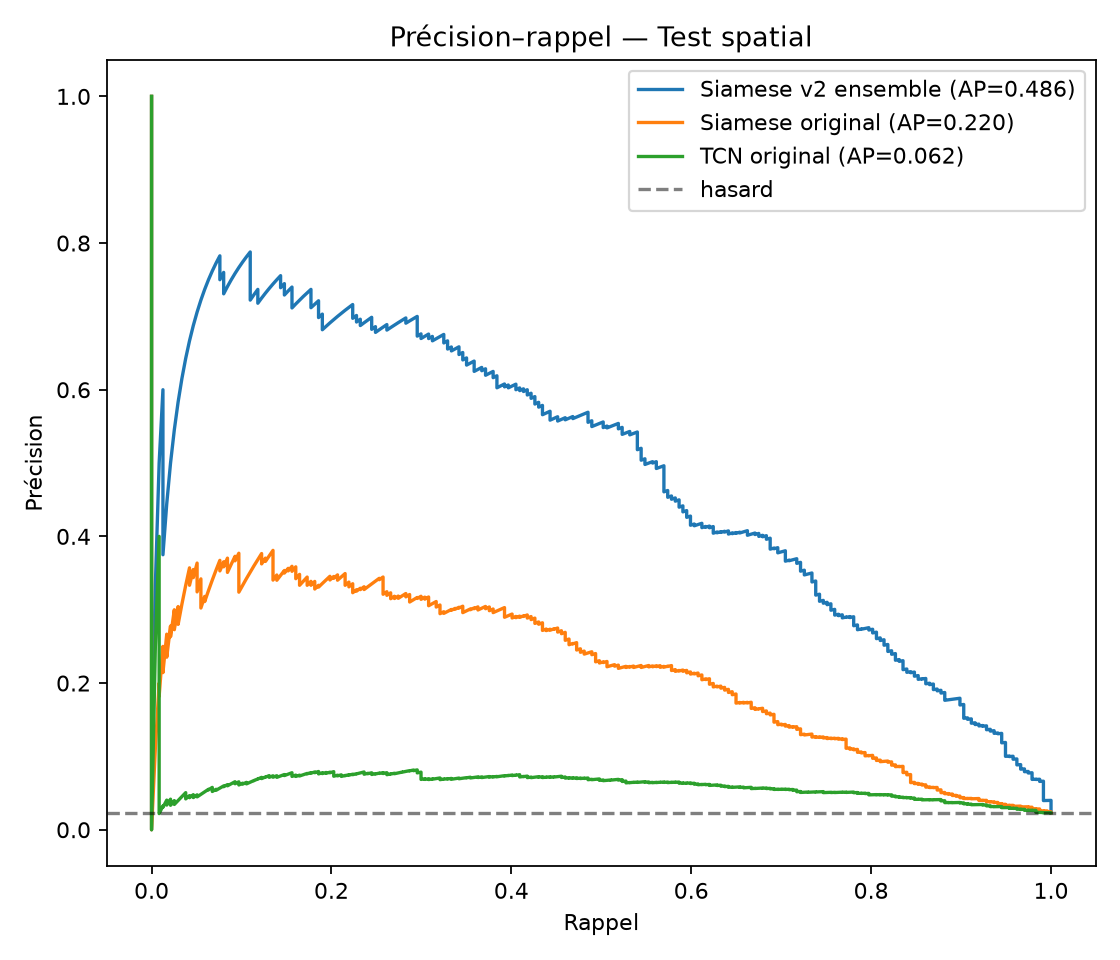
\includegraphics[width=0.86\columnwidth]{figures/pr_curves_original_vs_improved.png}
\caption{Courbes précision--rappel sur le test : Siamese v2\retro{} (ensemble), Siamese initial et TCN.}
\label{fig:pr2}
\end{figure}

\subsection{Seuils et budgets d'inspection}
\label{sec:op}
Le seuil doit suivre la capacité d'inspection plutôt qu'un F1 abstrait. La Table~\ref{tab:op} fixe, sur la validation, un
budget d'arbres à inspecter ou un rappel cible, puis applique ce seuil au test.

\begin{table}[t]
\centering\small
\caption{Points de fonctionnement\retro{} : seuils fixés sur validation, résultats sur test (rappel / précision, en \%).}
\label{tab:op}
\setlength{\tabcolsep}{3pt}
\begin{tabular}{@{}lccc@{}}
\toprule
Stratégie & Siamese v2 & Siamese init. & TCN \\
\midrule
Budget 2\,\% inspectés & 55 / 50 & 26 / 34 & 3 / 3 \\
Budget 5\,\% inspectés & 76 / 31 & 47 / 25 & 16 / 8 \\
Rappel cible $\geq$ 80\,\% : & & & \\
\quad arbres inspectés & 13,4\,\% & 30,8\,\% & 54,7\,\% \\
\quad rappel obtenu & 90\,\% & 85\,\% & 88\,\% \\
\bottomrule
\end{tabular}
\end{table}

En inspectant 2\,\% des arbres les mieux classés, le v2 retrouve plus de la moitié des disparitions, avec une alerte juste
sur deux. Pour un rappel d'au moins 80\,\%, il faut inspecter 13\,\% des arbres avec le v2, contre 31\,\% avec le Siamese
initial et 55\,\% avec le TCN.

\subsection{Contrôle de fuite spatiale}
\label{sec:leak}
Nous retirons du test les arbres situés à moins de $d$ mètres d'un arbre d'entraînement (Table~\ref{tab:leak}). La ROC-AUC
reste stable et la PR-AUC rapportée à la prévalence reste de 21 à 24 fois le hasard jusqu'à 50\,m. La baisse de la PR-AUC
brute suit surtout celle de la prévalence. À 100\,m, il ne reste que 13 positifs, effectif trop faible pour conclure. Enfin, un
modèle qui ne voit que l'image de 2019 reste au niveau du hasard (PR-AUC 0,039, section~\ref{sec:ablation}) : il n'existe pas de
raccourci contextuel (sol, parcelle, bord d'image) permettant de prédire la disparition.

\begin{table}[t]
\centering\small
\caption{Siamese v2\retro{} : test restreint aux arbres à plus de $d$ m de tout arbre d'entraînement.}
\label{tab:leak}
\setlength{\tabcolsep}{3.5pt}
\begin{tabular}{@{}rrrrrr@{}}
\toprule
$d$ (m) & Arbres & Pos. & ROC-AUC & PR-AUC & PR/prév. \\
\midrule
0 & 10\,205 & 237 & 0,961 & 0,486 & 20,9 \\
16 & 8\,989 & 178 & 0,963 & 0,426 & 21,5 \\
32 & 7\,537 & 108 & 0,965 & 0,339 & 23,7 \\
50 & 6\,065 & 61 & 0,955 & 0,234 & 23,3 \\
100 & 2\,760 & 13 & 0,877 & 0,026 & 5,5 \\
\bottomrule
\end{tabular}
\end{table}

\subsection{Validation croisée spatiale et taille des blocs}
\label{sec:cv}
Un seul test ne dit pas comment le modèle se comporte sur d'autres zones. Nous avons donc refait le découpage avec des blocs de
250\,m, 500\,m et 1\,km, chacun en 5 partitions géographiques (StratifiedGroupKFold sur les blocs). Pour chaque partition $k$,
le fold $k$ sert de test, le fold $k+1$ de validation (arrêt anticipé et seuil), et les trois autres d'entraînement, avec une
normalisation recalculée. Le Siamese~v2 est entraîné une fois par partition (une graine, sans ensemble), soit 15 modèles
(Table~\ref{tab:cv}).

\begin{table}[t]
\centering\small
\caption{Validation croisée spatiale\retro{} du Siamese v2 (5 partitions par taille de bloc, un modèle par partition) :
moyenne $\pm$ écart-type et [min ; max] sur les partitions.}
\label{tab:cv}
\setlength{\tabcolsep}{2.5pt}
\begin{tabular}{@{}lccc@{}}
\toprule
& 250\,m & 500\,m & 1\,km \\
\midrule
Blocs (total) & 363 & 109 & 35 \\
Blocs test avec positifs & 10,2 & 7,2 & 4,4 \\
PR-AUC test & $0{,}33\pm0{,}14$ & $0{,}32\pm0{,}13$ & $0{,}33\pm0{,}19$ \\
\quad [min ; max] & [0,19 ; 0,52] & [0,17 ; 0,53] & [0,14 ; 0,55] \\
ROC-AUC test & $0{,}92\pm0{,}03$ & $0{,}91\pm0{,}03$ & $0{,}91\pm0{,}04$ \\
F1 test & $0{,}35\pm0{,}11$ & $0{,}36\pm0{,}11$ & $0{,}36\pm0{,}15$ \\
PR-AUC / prévalence & $11\times$ & $11\times$ & $11\times$ \\
\bottomrule
\end{tabular}
\end{table}

Trois constats. (1) \textbf{La taille des blocs ne change pas la performance moyenne} (PR-AUC 0,32--0,33, ROC-AUC 0,91--0,92) :
séparer davantage l'entraînement et le test ne fait pas chuter le modèle, ce qui confirme l'absence de fuite spatiale
importante. Seule la dispersion augmente avec des blocs plus grands, car le test repose alors sur moins de zones.
(2) \textbf{La performance dépend fortement de la zone testée} : de 0,14 à 0,55 selon la partition, pour une prévalence
comparable. (3) \textbf{Le test d'origine est une zone plutôt favorable} : un modèle v2 seul y obtient 0,42 à 0,53 (Table~\ref{tab:v2}),
contre 0,33 en moyenne ici. L'estimation la plus prudente de la PR-AUC d'un modèle v2 seul sur une zone nouvelle du même
secteur est donc d'environ \textbf{0,33} (11 fois le hasard), et non 0,49. Toutes ces zones appartiennent au même secteur
de 35\,km$^2$ : la généralisation à d'autres régions, par exemple à des oliveraies marocaines aux conditions climatiques et
radiométriques différentes, reste non testée (section~\ref{sec:future}).

\subsection{Ablation : représentation ou architecture ?}
\label{sec:ablation}
Chaque variante du v2 est entraînée avec les mêmes hyperparamètres et trois graines (Table~\ref{tab:abl}, Figure~\ref{fig:abl}).
\begin{itemize}
\item \textbf{2019 seule} : niveau du hasard ; l'image initiale ne prédit pas la disparition.
\item \textbf{2021 seule} : l'image finale porte une partie du signal (couronne absente), mais la \emph{comparaison} avec 2019
ajoute $+0{,}12$ (validation) à $+0{,}15$ (test). La formulation bi-temporelle est justifiée.
\item \textbf{Sans partage des poids} : même performance avec deux fois plus de paramètres ; le partage est justifié (même
capteur, embeddings directement comparables).
\item \textbf{Niveaux de gris} : $-0{,}06$ en validation, sans effet net sur le test, très variable. L'apport de la couleur
est probable mais modéré ; l'essentiel du signal est structurel (forme et ombre de la couronne).
\item \textbf{Trois dates} : meilleure variante en validation ($+0{,}07$) comme en test ($+0{,}05$). L'image intermédiaire aide à
distinguer une disparition d'un artefact ponctuel.
\end{itemize}
\textbf{Déséquilibre et attention.} Sur la même partition et les mêmes graines (Table~\ref{tab:var}), la pondération des
positifs par $\sqrt{n_-/n_+}$ reste la meilleure stratégie. La perte focale donne un résultat équivalent en validation (0,292
contre 0,293, graine 0). Le rééchantillonnage équilibré des classes et le rééchantillonnage spatial (positifs pondérés par
l'inverse du nombre de positifs de leur bloc) sont moins bons : en répétant les mêmes positifs, ils favorisent le
surapprentissage. Ajouter une attention canal (SE) et un pooling par attention spatiale apporte un léger gain
(+0,01 en validation, +0,06 en test) pour 3\,\% de paramètres en plus. Ce gain reste dans la variabilité entre zones
(section~\ref{sec:cv}) et devra être confirmé.

\begin{table}[t]
\centering\small
\caption{Déséquilibre et attention\retro{} : PR-AUC moyenne $\pm$ écart-type (3 graines, partition d'origine).}
\label{tab:var}
\footnotesize\setlength{\tabcolsep}{2.5pt}
\begin{tabular}{@{}lcc@{}}
\toprule
Variante du Siamese v2 & Validation & Test \\
\midrule
Pondération $\sqrt{n_-/n_+}$ (référence) & 0,297 $\pm$ 0,011 & 0,434 $\pm$ 0,017 \\
Perte focale (graine 0) & 0,292 & -- \\
Rééchantillonnage équilibré & 0,284 $\pm$ 0,028 & 0,358 $\pm$ 0,048 \\
Rééchantillonnage spatial & 0,212 $\pm$ 0,031 & 0,364 $\pm$ 0,117 \\
Attention (SE + pooling spatial) & 0,306 $\pm$ 0,017 & 0,490 $\pm$ 0,019 \\
\bottomrule
\end{tabular}
\end{table}

\textbf{TCN contre MLP.} Avec trois dates, le champ récepteur du TCN (7 pas) couvre toute la série dès le premier bloc. Un MLP
sur les mêmes 12 valeurs obtient une PR-AUC comparable ($0{,}052\pm0{,}002$ contre $0{,}058\pm0{,}004$) : la convolution
temporelle n'apporte rien sur une série aussi courte. Ce résultat répond en partie à RQ1. Le Siamese initial et le TCN
diffèrent par leurs entrées autant que par leur architecture, mais l'ablation montre que les patches d'image à deux dates
portent l'essentiel du signal, que les statistiques résumées ne capturent pas.

\begin{table}[t]
\centering\footnotesize
\caption{Ablation\retro{} du Siamese v2 : PR-AUC moyenne $\pm$ écart-type (3 graines).}
\label{tab:abl}
\setlength{\tabcolsep}{2.5pt}
\begin{tabular}{@{}lrcc@{}}
\toprule
Variante & Param. & Validation & Test \\
\midrule
Référence (2019+2021) & 84\,721 & 0,297 $\pm$ 0,011 & 0,434 $\pm$ 0,017 \\
3 dates (2019--2021) & 88\,817 & \textbf{0,368 $\pm$ 0,031} & \textbf{0,484 $\pm$ 0,053} \\
Sans partage des poids & 157\,025 & 0,297 $\pm$ 0,017 & 0,454 $\pm$ 0,085 \\
Niveaux de gris & 84\,433 & 0,235 $\pm$ 0,013 & 0,446 $\pm$ 0,081 \\
2021 seule & 76\,529 & 0,175 $\pm$ 0,013 & 0,283 $\pm$ 0,043 \\
2019 seule (contrôle) & 76\,529 & 0,037 $\pm$ 0,004 & 0,039 $\pm$ 0,005 \\
\bottomrule
\end{tabular}
\end{table}

\begin{figure}[t]
\centering
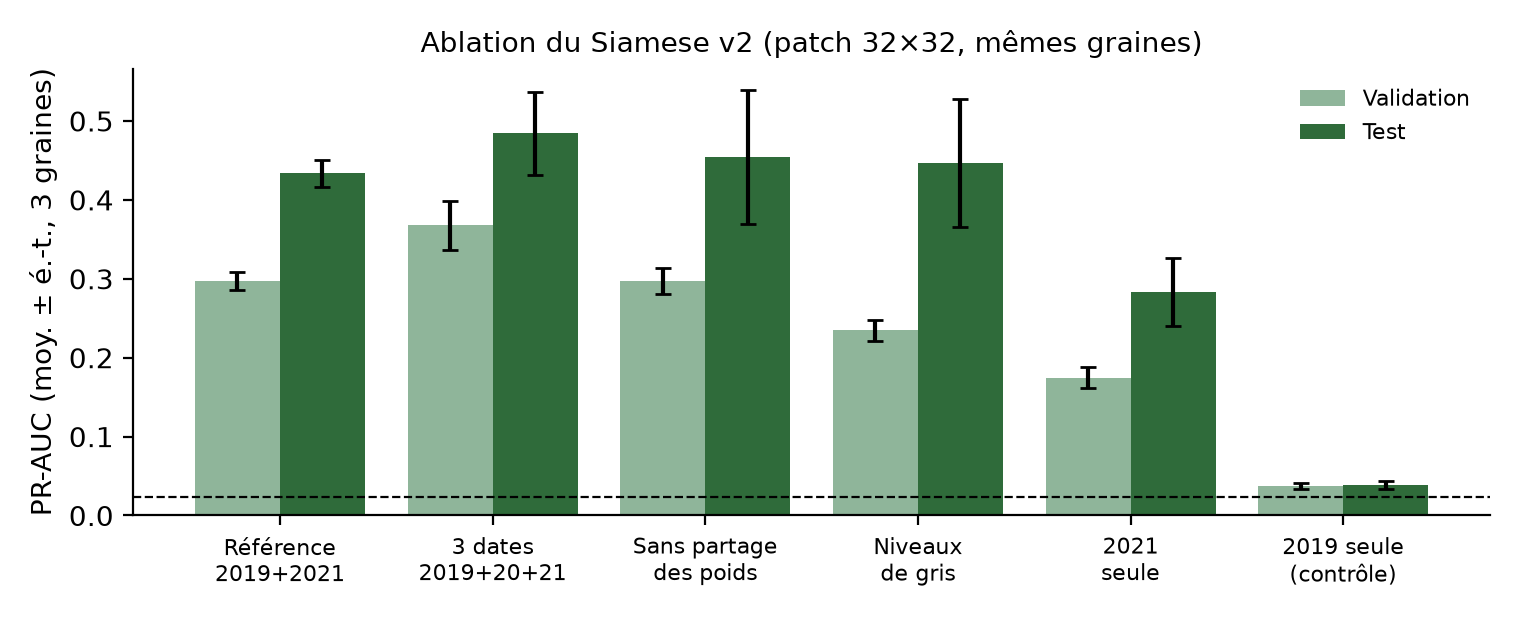
\includegraphics[width=\columnwidth]{figures/ablation_chart.png}
\caption{Ablation\retro{} : PR-AUC de validation et de test (moyenne $\pm$ écart-type, 3 graines). Pointillés : prévalence.}
\label{fig:abl}
\end{figure}

\subsection{Exemples réels multi-dates}
La Figure~\ref{fig:ex} montre un même arbre (cadre jaune) aux trois dates pour chaque type de décision du v2 au seuil 0,72.
Critère systématique : le 6\textsuperscript{e} score le plus extrême de chaque catégorie (pour éviter un cas limite
unique) ; le vrai négatif est tiré au hasard. Le vrai
positif montre une couronne nette en 2019--2020 puis absente en 2021. Le faux positif présente un fort changement d'éclairage
et de couleur du sol entre les dates sans disparition apparente. Le faux négatif est en bord de raster (pixels noirs). Ces cas
illustrent des hypothèses d'erreur, non des causes démontrées. OQDS ne contient pas de classe « dépérissant » : on ne peut
montrer que des arbres présents (négatifs) ou disparus (positifs). Un arbre d'apparence affaiblie mais toujours présent est un
négatif, et aucune de ces images ne permet de confirmer l'état sanitaire réel d'un arbre, sain ou malade.

\begin{figure}[t]
\centering
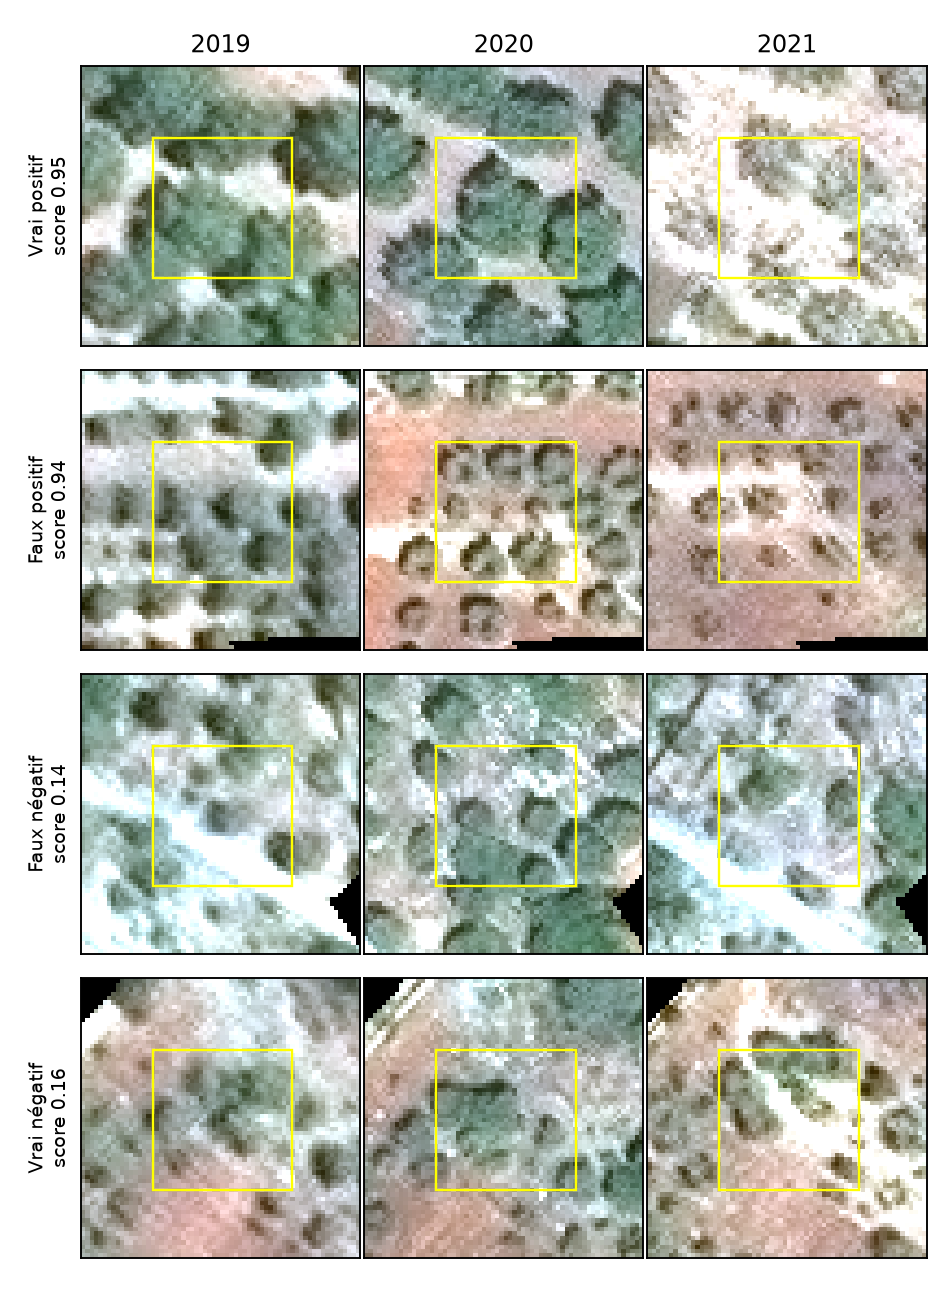
\includegraphics[width=0.80\columnwidth]{figures/examples_confusion_compact.png}
\caption{Exemples\retro{} réels (identifiants OQDS : VP 56610, FP 73872, FN 36678, VN 19267 ; score du v2 en marge, seuil
0,72). « Positif » = disparition apparente selon OQDS, sans preuve de maladie.}
\label{fig:ex}
\end{figure}

% ============================ 7. DISCUSSION ===============================
\section{Discussion}
\textbf{Réponses aux questions.} \textbf{RQ1} : oui, dans ce corpus. La comparaison de patches à deux dates surpasse les
indicateurs agrégés (Siamese 0,220 contre 0,062 au mieux en phase~1), et l'ablation attribue ce gain à la comparaison
d'images plutôt qu'à un raccourci. \textbf{RQ2} : le Siamese offre le meilleur compromis (3,3 alertes par disparition réelle en
phase~1) ; les méthodes à fort rappel (TCN, Isolation Forest) imposent 18 à 37 inspections par cas. \textbf{RQ3} : sensibilité
limitée aux pixels noirs stricts (ci-dessous), ce qui ne vaut pas robustesse générale.

\textbf{Portée du contrôle « pixels noirs ».} En test, 80,7\,\% des patches ne contiennent aucun pixel strictement noir ; le
Siamese y obtient un F1 de 0,333 (80 des 213 positifs retrouvés). Le groupe fortement noir ne contient que 13 positifs, aucun
détecté : l'effectif est trop faible pour conclure. Neutraliser les pixels transparents (alpha = 0) concerne 34 arbres et ne
change aucune décision (ROC-AUC de 0,873907 à 0,873756). Ce contrôle ne suffit pas à établir la robustesse aux ombres et à
l'éclairage.\label{sec:robust} Nous avons donc appliqué des perturbations synthétiques aux patches de test du Siamese~v2\retro{}
(Table~\ref{tab:robust}).

\begin{table}[t]
\centering\small
\caption{Robustesse\retro{} du Siamese v2 à des perturbations synthétiques appliquées à tous les arbres test (seuil fixe 0,72).}
\label{tab:robust}
\setlength{\tabcolsep}{3pt}
\begin{tabular}{@{}lrr@{}}
\toprule
Perturbation & PR-AUC & Alertes \\
\midrule
Aucune (référence) & 0,486 & 473 \\
2021 assombrie ($\times$0,8) & 0,482 & 118 \\
2019 et 2021 assombries ($\times$0,8) & 0,475 & 124 \\
Zone masquée noire 10$\times$10 px sur 2021 & 0,460 & 374 \\
Gamma 1,25 sur 2021 & 0,545 & 248 \\
Bord noir de 6 px sur 2021 & 0,394 & 135 \\
Ombre portée ($\times$0,5) sur 2019 & 0,401 & 662 \\
Contraste 2021 $\times$0,7 & 0,284 & 845 \\
2021 éclaircie ($\times$1,2) & 0,278 & 1\,067 \\
Ombre portée sur 2021 & 0,237 & 1 \\
\bottomrule
\end{tabular}
\end{table}

Le classement résiste à un assombrissement, à un masquage partiel et à une correction gamma. En revanche, \textbf{il se dégrade
fortement} quand 2021 est éclaircie, perd du contraste ou reçoit une ombre portée (PR-AUC de 0,24 à 0,28). Surtout, le nombre
d'alertes au seuil fixe varie de 1 à 1\,067 : le seuil n'est pas stable face à un changement radiométrique global.
L'augmentation utilisée à l'entraînement ($\pm$10\,\% de gain) est trop faible pour couvrir ces écarts. Ces perturbations,
appliquées uniformément, sont plus sévères que les écarts réels entre dates (section~3), mais elles montrent qu'une
normalisation radiométrique entre dates (par exemple un appariement d'histogrammes par bloc) et une augmentation plus forte
sont nécessaires avant tout usage. Les performances ne reposent donc pas sur les pixels noirs, mais elles restent sensibles à
l'éclairage.

\textbf{Menaces sur la validité.} Les principales limites viennent (i) de la cible indirecte : une disparition apparente n'est ni
une maladie ni une mort confirmée ; (ii) des observations spatialement groupées : les blocs empêchent le partage d'une même zone,
mais des blocs adjacents peuvent partager des dépendances visuelles et environnementales ; (iii) du biais de sélection modeste
introduit par les exclusions ; (iv) d'un unique test, déjà consulté, issu de la même région. Sans test géographique
indépendant, le classement observé doit être considéré comme exploratoire. La Table~\ref{tab:evidence} précise le niveau de
preuve de chaque conclusion.

\begin{table}[t]
\centering\small
\caption{Niveau de preuve des conclusions.}
\label{tab:evidence}
\setlength{\tabcolsep}{3pt}
\begin{tabular}{@{}L{4.6cm}L{3.2cm}@{}}
\toprule
Élément & Statut \\
\midrule
Classement des 5 méthodes (Tables~\ref{tab:main}--\ref{tab:burden}) & mesuré, confirmatoire \\
Siamese v2, graines, IC, budgets, fuite, ablation & mesuré, rétrospectif\retro{} \\
Exclusions, dépendance spatiale & audité \\
Sources auxiliaires (NEON, CrownsDb, Hyperspectral) & auditées, non équivalentes \\
Robustesse à l'éclairage et aux ombres & testé (synthétique) : sensible \\
Robustesse au recalage géométrique & non testé \\
Généralisation entre zones du même secteur & mesuré, rétrospectif\retro{} (section~\ref{sec:cv}) \\
Généralisation à une nouvelle région & proposé (section~\ref{sec:future}) \\
Diagnostic sanitaire, vérité terrain & indisponible \\
Latence d'un service API & non mesuré \\
\bottomrule
\end{tabular}
\end{table}

\textbf{Limites de l'exploration.} La recherche d'hyperparamètres reste restreinte : 3 configurations par réseau en phase~1,
puis 4 configurations, 6 variantes d'ablation, 3 stratégies de déséquilibre et une variante à attention en phase~2, toutes sur
CPU. Le taux d'apprentissage, la taille de lot et la profondeur n'ont pas été balayés systématiquement. Les architectures de
détection de changement de type U-Net ou Transformers spatio-temporels n'ont pas été testées : elles produisent des cartes
\emph{par pixel} et demandent des masques de changement, ou de longues séries, que le corpus ne fournit pas (une étiquette
par arbre, trois dates). Enfin, l'étude par catégorie de changement (disparition complète, couronne réduite, végétation
voisine modifiée, changement d'apparence sans disparition) est impossible sans annotation de ces catégories : OQDS ne distingue
que présent et disparu. Elle fait partie du protocole futur.

\textbf{Sources auxiliaires.} L'expérience hyperspectrale (régression logistique sur composantes principales, validation croisée
stratifiée) donne une ROC-AUC de 0,798 et une PR-AUC de 0,262 sur 76 observations, dont 6 positives. Elle est exploratoire et
non comparable aux scores OQDS. NEON et CrownsDb ne fournissent pas d'étiquette temporelle de santé et ne peuvent pas servir de
test externe.

\textbf{Modèle retenu.} Le choix repose sur la validation : le Siamese v2 y obtient 0,314, contre 0,167 pour le Siamese initial et
0,054 au mieux pour les méthodes non neuronales. Il accepte directement deux images d'un arbre, ce qui correspond à l'usage
prévu. La variante à trois dates, meilleure en validation dans l'ablation, est la prochaine évolution. Ces choix devront être
confirmés sur un test nouveau.

% ===================== INTÉGRATION ET REPRODUCTIBILITÉ ====================
\section{Intégration logicielle et reproductibilité}
\label{sec:api}
\textbf{Architecture prévue (conception, non déployée).} Le modèle sera servi par un microservice Python \textbf{FastAPI}
(« olv6-inference »), appelé par les services \textbf{Spring Boot} d'OliveSmart. Au démarrage, le service charge une seule fois
le checkpoint de l'ensemble (\texttt{siamese\_ensemble\_best.pt}), les statistiques de normalisation et le seuil gelé, en mode
évaluation. La version du modèle est l'empreinte SHA-256 du fichier, et un échec de chargement rend le service indisponible
plutôt que de répondre avec un autre modèle. Les images voyagent de deux façons : soit des patches 32$\times$32 encodés en PNG
base64 dans le JSON (requêtes unitaires), soit, pour les traitements par lot, des références vers des rasters déposés sur un
stockage partagé, le service découpant lui-même les patches à partir des coordonnées. Côté Spring Boot, un client REST
(WebClient) appelle le service avec un délai maximal, et les traitements par lot passent par une file de tâches asynchrone.

\begin{table}[t]
\centering\small
\caption{Points d'accès REST prévus du service d'inférence.}
\label{tab:api}
\setlength{\tabcolsep}{3pt}
\begin{tabular}{@{}lL{5.0cm}@{}}
\toprule
Point d'accès & Rôle \\
\midrule
\texttt{GET /health} & état du service et version du modèle chargé \\
\texttt{GET /model} & version, seuil, taille d'entrée, métriques de validation, date d'entraînement \\
\texttt{POST /predict} & un arbre : coordonnées et deux patches (ou références de rasters) \\
\texttt{POST /predict/batch} & liste d'arbres ou emprise ; traitement asynchrone avec identifiant de tâche \\
\texttt{GET /jobs/\{id\}} & état et résultats d'un traitement par lot \\
\bottomrule
\end{tabular}
\end{table}

\textbf{Coût de calcul.} La Table~\ref{tab:bench} compare les méthodes sur la même machine (CPU Intel, 32 threads logiques,
PyTorch 2.15 CPU, aucun autre calcul en cours ; patches déjà extraits). Le Siamese~v2 seul répond en 2,7\,ms pour un arbre et
traite le test complet en 3\,s ; l'ensemble de 5 modèles multiplie ces temps par 5. Même ainsi, un secteur de 10\,000 arbres
est traité en moins de 15\,s : le coût de calcul n'est pas un obstacle pour un usage par lot.

\begin{table}[t]
\centering\small
\caption{Coût de calcul dans des conditions identiques : latence d'un arbre (1 thread, médiane de 300 appels) et durée
pour les 10\,205 arbres test (8 threads). Isolation Forest : nombre de nœuds au lieu de paramètres.}
\label{tab:bench}
\footnotesize\setlength{\tabcolsep}{2.5pt}
\begin{tabular}{@{}lrrrr@{}}
\toprule
Méthode & Param. & Poids & 1 arbre & 10\,205 arbres \\
\midrule
Seuil & 1 & $<$1\,ko & 0,05\,ms & 0,6\,ms \\
CUSUM & 2 & $<$1\,ko & 0,44\,ms & 0,9\,ms \\
TCN & 1\,081 & 9\,ko & 0,41\,ms & 8\,ms \\
Isolation Forest & 113\,890 & 9,7\,Mo & 36,6\,ms & 0,37\,s \\
Siamese initial & 7\,201 & 32\,ko & 0,47\,ms & 0,21\,s \\
Siamese v2 (1 modèle) & 84\,721 & 0,34\,Mo & 2,7\,ms & 2,9\,s \\
Siamese v2 + attention & 87\,614 & 0,35\,Mo & 3,3\,ms & 3,2\,s \\
Siamese v2 (ensemble 5) & 423\,605 & 1,7\,Mo & 14,7\,ms & 14,8\,s \\
\bottomrule
\end{tabular}
\end{table}

\noindent Réponse de \texttt{POST /predict} (exemple de format) :
{\footnotesize
\begin{verbatim}
{ "tree_id": "26925", "x": 708258.5, "y": 4513499.8,
  "crs": "EPSG:32633",
  "dates": ["2019", "2021"],
  "score": 0.83, "threshold": 0.72,
  "predicted_class": "disparition_apparente",
  "model_version": "siamese_v2_ens5@3f9a1c2e",
  "patch_source": "WV2_RGB_0.5m",
  "warnings": ["pixels_noirs_2021 > 20 %"] }
\end{verbatim}
}
\noindent La classe renvoyée est toujours « disparition apparente » ou « pas de disparition », jamais « malade » ou « mort ».
Le champ \texttt{warnings} signale les entrées hors du domaine d'entraînement (pixels noirs, écart radiométrique fort,
section~\ref{sec:robust}). Aucun déploiement HTTP n'a encore été testé sous charge : la Table~\ref{tab:bench} donne des temps
de calcul du modèle, pas des latences de service.

\textbf{Reproductibilité.} Le code, les configurations et les résultats sont versionnés dans le dépôt GitHub du projet
(\texttt{Project-JEE-DL}). On y trouve l'environnement (Python 3.12.13, PyTorch 2.15 CPU, \texttt{requirements.txt}),
la graine de base (20261106, avec des décalages fixes par graine), les configurations retenues
(\texttt{selected\_configurations.json}, \texttt{frozen\_choices.json}), les checkpoints, les prédictions de test et
l'historique de chaque entraînement. Les scripts s'exécutent dans cet ordre : \texttt{audit\_datasets}, \texttt{prepare\_oqds},
\texttt{train\_evaluate} (phase 1), puis \texttt{train\_improved}, \texttt{analyses\_remarques}, \texttt{experiments\_ablation},
\texttt{experiments\_spatial}, \texttt{analyses\_complementaires} et \texttt{benchmark\_compute} (phase 2). Le rechargement de
l'ensemble v2 reproduit ses scores à $1{,}4\cdot10^{-7}$ près. Le mode « consultation » du notebook a été réexécuté dans un
noyau neuf sans erreur. En revanche, la chaîne complète n'a pas été réexécutée dans un environnement isolé : c'est la prochaine
vérification à faire. Les données brutes (5,8\,Go) ne sont pas versionnées et doivent être téléchargées depuis leurs sources.

% =========================== 8. FUTUR PROTOCOLE ===========================
\section{Protocole de validation futur}
\label{sec:future}
Le prochain test devra être fixé \emph{avant} toute expérimentation, avec :
\begin{enumerate}
\item une région ou une exploitation indépendante, scellée jusqu'au gel du modèle et du seuil (validation de type
\emph{leave-one-region-out}) ;
\item une zone tampon d'au moins 50\,m entre entraînement et test~\cite{valavi} ;
\item un critère primaire unique (PR-AUC), des budgets d'inspection (2\,\% et 5\,\%), 5 graines et des IC95 par blocs, avec
le nombre de blocs et de positifs ;
\item des règles d'exclusion écrites à l'avance et appliquées sans regarder les étiquettes ;
\item une vérification terrain d'un échantillon stratifié : toutes les alertes d'un budget de 2\,\% et un tirage aléatoire de
non-alertes, contrôlés par visite ou drone, pour estimer précision et rappel réels sur le terrain ;
\item lors de cette visite, une annotation de la cause : arbre arraché, mort sur pied, fortement dépérissant, couronne réduite
ou simple différence d'acquisition. Ces catégories permettront d'évaluer le modèle par type de changement ;
\item idéalement, une bande proche infrarouge calibrée, seule à même de détecter un \emph{dépérissement} (couronne présente mais
affaiblie), invisible en RGB 8 bits.
\end{enumerate}
Le test actuel, déjà consulté, reste réservé au diagnostic rétrospectif.

% ============================ 9. CONCLUSION ===============================
\section{Conclusion}
Nous avons comparé cinq méthodes de détection de la disparition apparente d'oliviers sur un test spatial commun. Dans la
phase pré-spécifiée, le Siamese CNN obtient la meilleure PR-AUC (0,220), la meilleure ROC-AUC (0,874) et le meilleur F1
(0,322), mais ne retrouve que 82 des 237 positifs pour 190 fausses alertes. Des analyses rétrospectives montrent que ce modèle
était sous-entraîné : une version révisée atteint 0,486 de PR-AUC et 72\,\% de rappel sur le test d'origine, mais environ 0,33
en moyenne sur 15 partitions géographiques, ce qui reste 11 fois mieux que le hasard. L'ablation attribue le gain à la
comparaison des deux dates. Ces résultats soutiennent une préférence de modèle relative, pas un système autonome de diagnostic.

Trois problèmes scientifiques distincts doivent rester séparés. (1) \textbf{Détecter la disparition} d'une couronne entre deux
dates : c'est ce que ce travail mesure, avec des images RGB et l'étiquette OQDS. (2) \textbf{Identifier le dépérissement}
d'un arbre encore présent (couronne éclaircie, vigueur réduite) : cela demande une étiquette graduée et, idéalement, un proxy
infrarouge calibré, absents ici. (3) \textbf{Diagnostiquer une maladie} (par exemple \emph{Xylella} ou \emph{Verticillium}) :
cela exige une vérité terrain biologique (prélèvement, analyse de laboratoire) qu'aucune image seule ne remplace. Nos
résultats ne portent que sur le premier problème. La cible est indirecte, le test est spatialement groupé et déjà consulté, et
le modèle reste sensible à l'éclairage. Une validation géographique pré-spécifiée et une vérité terrain indépendante sont
nécessaires avant tout usage opérationnel.

% ============================ RÉFÉRENCES =================================
{\footnotesize
\begin{thebibliography}{99}
\setlength{\itemsep}{0pt}
\bibitem{oqds} Crecco et al., article de données OQDS, \emph{Data in Brief}, 2025. doi:10.1016/j.dib.2025.111615.
\bibitem{lin} Lin et al., cartographie d'oliviers par télédétection, \emph{ISPRS J. Photogramm. Remote Sens.}, 2024. doi:10.1016/j.isprsjprs.2024.08.003.
\bibitem{raouhi} E. M. Raouhi et al., « Optimization techniques in deep convolutional neuronal networks applied to olive diseases classification », \emph{Artif. Intell. Agric.}, vol.~6, pp.~77--89, 2022. doi:10.1016/j.aiia.2022.06.001.
\bibitem{page} E. S. Page, « Continuous inspection schemes », \emph{Biometrika}, vol.~41, pp.~100--115, 1954.
\bibitem{iforest} F. T. Liu, K. M. Ting, Z.-H. Zhou, « Isolation Forest », \emph{IEEE ICDM}, 2008.
\bibitem{bromley} J. Bromley et al., « Signature verification using a Siamese time delay neural network », \emph{NeurIPS}, 1993.
\bibitem{daudt} R. C. Daudt, B. Le Saux, A. Boulch, « Fully convolutional Siamese networks for change detection », \emph{IEEE ICIP}, 2018. doi:10.1109/ICIP.2018.8451652.
\bibitem{bai} S. Bai, J. Z. Kolter, V. Koltun, « An empirical evaluation of generic convolutional and recurrent networks for sequence modeling », arXiv:1803.01271, 2018.
\bibitem{roberts} D. R. Roberts et al., « Cross-validation strategies for data with temporal, spatial, hierarchical, or phylogenetic structure », \emph{Ecography}, vol.~40, pp.~913--929, 2017. doi:10.1111/ecog.02881.
\bibitem{valavi} R. Valavi, J. Elith, J. J. Lahoz-Monfort, G. Guillera-Arroita, « blockCV: An R package for generating spatially or environmentally separated folds for k-fold cross-validation of species distribution models », \emph{Methods Ecol. Evol.}, vol.~10, no.~2, pp.~225--232, 2019. doi:10.1111/2041-210X.13107.
\bibitem{saito} T. Saito, M. Rehmsmeier, « The precision-recall plot is more informative than the ROC plot when evaluating binary classifiers on imbalanced datasets », \emph{PLoS ONE}, 10(3), 2015. doi:10.1371/journal.pone.0118432.
\bibitem{neon} weecology, « NEON tree crowns », Hugging Face Datasets.
\bibitem{hyper} « Olive hyperspectral stress », Zenodo, record 10336545.
\bibitem{crowns} Y. Hnida et al., « OliveTreeCrownsDb », Mendeley Data, v2, 2024. doi:10.17632/xym8rd2srf.2.
\end{thebibliography}
}

\end{document}
